\documentclass[11pt]{article}
\usepackage[utf8]{inputenc}
\usepackage{graphicx} % Allows you to insert figures
\usepackage{amsmath} % Allows you to do equations
\usepackage{fancyhdr} % Formats the header
\usepackage{hyperref}
\usepackage{fancyhdr}%header and footer
\usepackage{algorithm,algpseudocode}
\usepackage{amssymb}
\usepackage{url}
\pagestyle{fancy}
\fancyhead{}
\fancyfoot{}
\fancyfoot[R]{\thepage}
\usepackage[a4paper, inner=1.7cm, outer=2.7cm, top=2cm, bottom=2cm, bindingoffset=1.2cm]{geometry} % Formats the paper size, orientation, and margins
\linespread{1.25} % about 1.5 spacing in Word
\setlength{\parindent}{0pt} % no paragraph indents
\setlength{\parskip}{1em} % paragraphs separated by one line

\begin{document}

%START THE TITLE PAGE
\begin{titlepage}
\begin{center}
    
\includegraphics[width=8cm]{images/logo.jpg}
\end{center}

\begin{center}
\begin{Large}
\textbf{SOEN 6011 : SOFTWARE ENGINEERING PROCESSES} \\
\vspace*{0.1in}
\textbf{SUMMER 2022}\\
\vspace*{0.9in}
\end{Large}
\begin{Large}
\textbf{ETERNITY}\\
\vspace*{0.1in}
Instructor: PANKAJ KAMTHAN \\
\vspace*{0.9in}
\begin{Huge}
\textbf{Project Report}\\
\vspace*{0.9in}
\end{Huge}
\end{Large}

\begin{center}
    \line(1,0){300}\\
    \textbf{Student Name: Yun Ni\\
    Student ID: 40179775}\\
    \textbf{July, 2022}\\
    \line(1,0){300}\\
    \vspace*{0.5in}
    \textbf{Overleaf}:\url{https://www.overleaf.com/project/62ccdd9901199fc8cfc53a1f} \\
    \textbf{Github}: \url{https://github.com/ninanee/SOEN6011_Project} 
\end{center}
\end{center}

\end{titlepage}
%END THE TITLE PAGE

\newpage
\section{PROBLEM 1}\label{problem1}
\subsection{Introduction}
The function $f(x) = ab^x$ is an exponential function where $a\neq0, b>0$ and $b\neq1$. In this exponential function, $a$ is a initial quality, $b$ is the growth factor or decay factor and $c$ is the exponent. The function is called exponential because it has the input variable in the exponent and we can repeatedly multiplying by $b$~\cite{browder2012mathematical}.

\subsection{Domain}
The domain of this function is given by all the values that $x$ can take. If $b$ is a positive real number other than 1 and $a> 0$, $x$ can take any value.\\
Therefore, the domain is \textbf{$x\in R$}.

\subsection{Co-domain}
The co-domain is given by the dependent values of the variable $y$, where $y = ab^x$. If we evaluate $f(-\infty)$ then $y$ tends to zero. Besides, if we evaluate $f(\infty)$ then $y$ tends to infinity\cite{Anu:2013}.
Therefore, the co-domain is $(0, \infty)$.

\subsection{Characteristics}
\begin{itemize}
    \item Growth: if $b>0$, the function represents exponential growth which is a function increasing at a constant percentage. It is shown on the right hand side of Figure \ref{fig:my_label}.
    \item Decay: if $0<b<1$, the function represents exponential decay which is a function decreasing at a constant percentage. It is shown on the left hand side of Figure \ref{fig:my_label}.
    \item Invective and Subjective: this function is subjective since for every $y$, there is an $x$ such that $f(x) = y$, and it is not an invective function.
\end{itemize}

\begin{figure}[h]
    \centering
    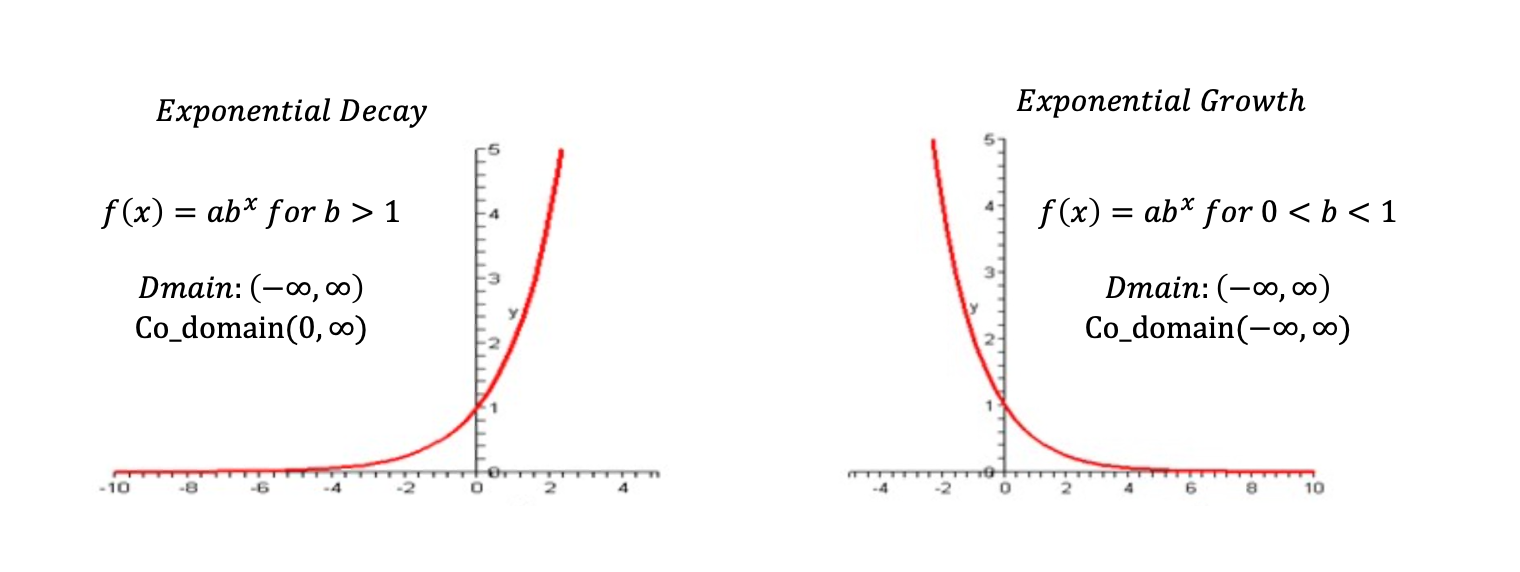
\includegraphics[width=12cm]{images/Function.png}
    \caption{The graph representation of $f(x) = ab^x$}
    \label{fig:my_label}
\end{figure}

\subsection{Context of Use Model}
The context of use model for the exponential function calculator is represented by the UML Class Diagram as Figure \ref{fig:context}.
\begin{figure}[h]
    \centering
    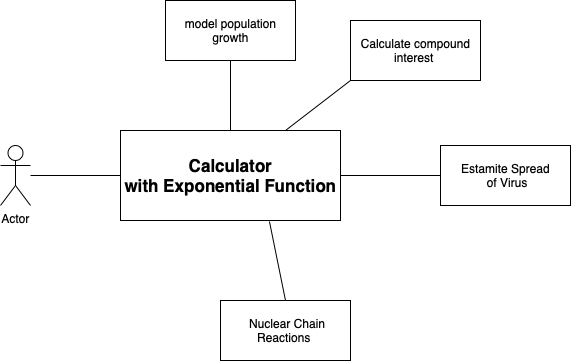
\includegraphics[width=8cm]{images/Context_diagram.png}
    \caption{The Context Diagram for exponential function calculator}
    \label{fig:context}
\end{figure}

As the figure shows above, the calculator can be used in both technical and non-technical environment \cite{zelen1966application}\cite{lebanon2001boosting}.
\begin{itemize}
    \item Technical Environment: help scientists model the number of new infections over time.
    \item Non-technical environment: help a student calculate the retirement account.
\end{itemize}

\section{PROBLEM 2}\label{problem2}
This section presents the assumptions and requirements for implementing $f(x)=ab^x$.
\subsection{Assumptions}
\begin{enumerate}
    \item The Function will accept only real numbers as inputs.
    \item The Function will be able to handle entry value of double-precision floating-point.
\end{enumerate}

\subsection{Requirements}
\begin{center}
    \begin{tabular}{|p{3cm}|p{11cm}| }
    \hline
    \textbf{Identification} &  FR1 \\ \hline 
    \textbf{Type} & Functional Requirement\\ \hline 
    \textbf{Priority} & High  \\ \hline
    \textbf{Difficulty} & Medium  \\ \hline
    \textbf{Description} & System needs to take inputs $x, a, b$ to give an output of $ab^x$. Besides, needs to define the constrains that $a\neq0, b > 0, b \neq 1$. Because, when $a=0$ or $b=0$, the function will be simplified to $y = f(x) = 0$. In addition, when $b = 1$,  the function will be simplified to $y = f(x) = a$, like a constant function.\\ \hline
\end{tabular}
\end{center}

\begin{center}
    \begin{tabular}{|p{3cm}|p{11cm}| }
    \hline
    \textbf{Identification} &  FR2 \\ \hline 
    \textbf{Type} & Functional Requirement\\ \hline 
    \textbf{Priority} & High  \\ \hline
    \textbf{Difficulty} & Medium  \\ \hline
    \textbf{Description} & Function $ab^x$ does not depend on any other functions like built-in or library functions.\\ \hline
\end{tabular}
\end{center}

\begin{center}
    \begin{tabular}{|p{3cm}|p{11cm}| }
    \hline
    \textbf{Identification} &  FR3 \\ \hline 
    \textbf{Type} & Functional Requirement\\ \hline 
    \textbf{Priority} & High  \\ \hline
    \textbf{Difficulty} & Medium  \\ \hline
    \textbf{Description} & Users can give an input from all real numbers for $x$.\\ \hline
\end{tabular}
\end{center}

\begin{center}
    \begin{tabular}{|p{3cm}|p{11cm}| }
    \hline
    \textbf{Identification} &  FR4 \\ \hline 
    \textbf{Type} & Functional Requirement\\ \hline 
    \textbf{Priority} & High  \\ \hline
    \textbf{Difficulty} & Easy  \\ \hline
    \textbf{Description} & When users give other inputs than a number like a string, the system should not accept and should show the exception properly.\\ \hline
\end{tabular}
\end{center}

\begin{center}
    \begin{tabular}{|p{3cm}|p{11cm}| }
    \hline
    \textbf{Identification} &  FR5 \\ \hline 
    \textbf{Type} & Functional Requirement\\ \hline 
    \textbf{Priority} & High  \\ \hline
    \textbf{Difficulty} & Easy  \\ \hline
    \textbf{Description} & When users give inputs does not specify all there inputs like $a, b, x$, the system should not accept and throw an error.\\ \hline
\end{tabular}
\end{center}

\begin{center}
    \begin{tabular}{|p{3cm}|p{11cm}| }
    \hline
    \textbf{Identification} &  FR6 \\ \hline 
    \textbf{Type} & Functional Requirement\\ \hline 
    \textbf{Priority} & High  \\ \hline
    \textbf{Difficulty} & Easy  \\ \hline
    \textbf{Description} &Ensure the accuracy of decimal operations to the power of decimals.\\ \hline
\end{tabular}
\end{center}

\section{PROBLEM 3}\label{problem3}
This section presents the pseudo-code and algorithm for implementing $f(x)=ab^x$.
\subsection{Algorithm 1: Iterative}
The interactive algorithm can execute the steps in number of iterations, using the loop. We can track the result in a variable called prod, which is initially set to 1 and then use loop from 1 to x number of times. By incriminating by one on each iteration, we multiply prod by b. At the end of the loop value of prod is equal to $b^x$ then return the result of $a * prod$\cite{xu2015application}.

\begin{algorithm}
  \caption{Iterative algorithm for calculating $f(x) = ab^x$}
  \begin{algorithmic}[1]
  \Require $a \neq 0$ and $b > 0$ and $b \neq 1$ 
    \Function\textbf{\textbf{exponent\_iterative(a,b,x)}}\\
    \textbf{in: }double number x, a, b\\
    \textbf{out: }double number prod
    \State $prod \gets 1$
    \State $temp \gets 1$
    \For{\texttt{$temp \leq x$}}
        \qquad \State $prod \leftarrow prod*b$
        \qquad \State $temp \leftarrow temp+1$
    \EndFor
    \State $prod \gets prod*a$
    \State return $prod$
    \EndFunction
  \end{algorithmic}
\end{algorithm}

\begin{center}
\begin{tabular}{|p{7cm}|p{7cm}|}
\hline
     \textbf{Advantages} & \textbf{Disadvantages}\\ \hline
     Easy to implement, since it uses looping structure. & If the condition fails, the iteration terminates the execution of the program.\\ \hline
     Tracing the iterative algorithm is easy. & It is not very efficient in terms of time since the time complexity is $O(n)$ for a larger input\cite{xu2015application}. \\ \hline
     Could avoid memory overflow of input. & Can not calculate decimal inputs properly in this case.\\ \hline
\end{tabular}
\end{center}

\subsection{Algorithm 2: Recursive}
A recursive function calls by itself during the execution of the program, until the base conditions are met\cite{haberman2002case}. By defining a helper function called exponent\_helper which calculates $b^x$ in different conditions. With the helper function, we multiply the result to the value of input $a$ and return it to the user.

\begin{algorithm}
  \caption{Recursive algorithm for calculating $f(x) = ab^x$}
  \begin{algorithmic}[1]
  \Require $a \neq 0$ and $b > 0$ and $b \neq 1$ 
   \Function\textbf{\textbf{exponent\_recursive(a,b,x)}}\\
    \textbf{in: }double number x, a, b\\
    \textbf{out: }double number prod
    \State $power \gets exponent\_helper(b,x)$
    \State $prod \gets power * a$
    \State return $prod$
    \EndFunction
  \end{algorithmic}
\end{algorithm}

\begin{algorithm}
  \begin{algorithmic}[1]
   \Function\textbf{\textbf{exponent\_helper(b,x)}}\\
   \textbf{in: }number x, b\\
   \textbf{out: }double number prod
   \If{$x < 0$}
   \State $b \gets 1.0 / b$
   \State $x \gets -x$ 
   \State return $exponent\_helper(b, x)$ 
   \ElsIf{$x = 0$}
     \State return $1.0$
   \ElsIf{ $x = 1$}
    \State return $b$
   \ElsIf{$x \mod  2 = 0$}
    \State $b \gets b * b$ 
    \State $x \gets x / 2$ 
    \State return $exponent\_helper(b, x)$
    \Else
    \State $b \gets b * b$ 
    \State $x \gets x - 1$ 
    \State $x \gets x / 2$ 
    \State return $exponent\_helper(b, x)$
    \EndIf 
   \EndFunction
  \end{algorithmic}
\end{algorithm}

\begin{center}
\begin{tabular}{|p{7cm}|p{7cm}|}
\hline
     \textbf{Advantages} & \textbf{Disadvantages}\\ \hline
     The time complexity of the defined recursive algorithms above is $O(\log n)$. & Recursive algorithm is not easy to debug since it calls itself.\\ \hline
     Recursive algorithms is easier to maintain than loop\cite{karigl1981recursive}. & Recursive algorithm needs the system continuously allocates memory, might lead stack overflow\cite{haberman2002case} \\ \hline
      & Can not calculate decimal inputs properly in this case.\\ \hline
\end{tabular}
\end{center}

\subsection{Algorithm 3: Taylor Series for calculating $f(x) = ab^x$}
For calculating the exponential function $f(x) = ab^x$ more properly, we can use Taylor Series algorithm. When $x$ is a decimal, Taylor Series can calculate $\ln(x)$ and $e^x$ with a high precision, since the formula can be changed to $b^x = e^{b\ln b}$. When $x$ is an integer, if $x$ is an even number, $b^x$ can be decomposed to $(b^2) (x/2)$; if $x$ is an odd number, $b^x$ can be decomposed to $b\cdot ((b^2) ((x-1)/2)$. And then continue to decompose until the exponent part is equal to one\cite{abad2012algorithm}.

\begin{algorithm}
\caption{Exponentiation by Taylor Series\cite{Anu:Stack_Overflow}}\label{exp1}
\begin{algorithmic}[1]
\Require $a \neq 0$ and $b > 0$ and $b \neq 1$ 
\Function{logarithm}{$n$}\Comment{algorithm for $log(n)$}
\State $sum\gets 0$
\While{$n > 1$}
    \State $n\gets n/e$\Comment{e is a constant approximately equal to 2.71828}
    \State $x \gets x + 1 $
\EndWhile \\
\Return $x$
\EndFunction

\Function{exponential}{$b$}\Comment{algorithm for $e^b$}
\State $sum\gets 1$
\State $n\gets 10$
\For{$i\gets n-1$, 1}
\State $sum\gets 1+ b * sum / i$
\EndFor \\
\Return $sum$
\EndFunction

\State $\log b \gets $\Call{logarithm}{$b$}
\State $result \gets $\Call{exponential}{$x* \log b$}
\State $result \gets $\Call{$a\cdot$}{$result$}
\end{algorithmic}
\end{algorithm}

\begin{center}
    \begin{tabular}{|p{7cm}|p{7cm}|}\hline
        \textbf{Advantages} & \textbf{Disadvantages}\\\hline
        The Taylor Series is very useful for derivations and can calculate even the most complex functions. & The algorithm could be very complex with deriving.\\\hline The Taylor Series can be used to get theoretical error bounds and estimate the value of any input\cite{hariharan2010comparative}.  & The expansion point might lead truncation errors.\\\hline
    \end{tabular}
\end{center}
\subsection{Conclusion}
For a function, the accuracy is the most significant factor, since a wrong output is worse than a blank. The iterative and recursion algorithms can not calculate the decimal part of $f(x) = ab^x$ with high precision, therefore, my decision is to use Taylor Series algorithm to implement the function. It could runs more efficiently and provide results with high accuracy.

\section{ PROBLEM 4}
\subsection{Debugger}
You must use a debugger. You must include one or more snapshots of the debugger you used to show its usage. Give a brief description, not exceeding one page, of the debugger you used, including its advantages and disadvantages.

\subsection{The Quality Attributes}
Your Java source code must aim to be space-efficient, portable, and maintainable. Your Java program must aim to be correct, robust, time-efficient, and usable. State explicitly the effort made towards achieving each of these quality attributes

\subsection{Checkstyle}
You must use a tool, such as Checkstyle, to check the pragmatic quality of your Java source code. You must include one or more snapshots of the tool you used to show its usage. Give a brief description, not exceeding one page, of the tool you used, including its advantages and disadvantages. 

\newpage
\bibliographystyle{plain}
\bibliography{bibliography.bib}
\end{document}